%%%%%%%%%%%%%%%%%%%%%%%%%%%%%%%%%%%%%%%%%%%%%%%%%%%%%%%%%%%%%%%%%%%%%%%%
\chapter{Background}
%%%%%%%%%%%%%%%%%%%%%%%%%%%%%%%%%%%%%%%%%%%%%%%%%%%%%%%%%%%%%%%%%%%%%%%%
In this chapter, we first outline the aims and approaches of solving the object
detection task. We then describe the fundamentals of deep learning for a better
understanding of our chosen object detection models.

\section{Object Detection}

Object detection aims to locate objects in a given image and assign them to
their \bld{class} (also called category or label). For illustration see Figure
\ref{fig:od}. Generally, the task can be broken down into three steps:
\bld{informative region selection}, \bld{feature extraction}, and
\bld{classification}. In the first step, the method has to determine regions to
which we apply the feature extraction. The feature extractor outputs a semantic
numerical representation for each selected region is then used to predict the
target's class. Note that, these steps are not fixed and the pipeline can vary.

\begin{figure}[h]
    \centering
    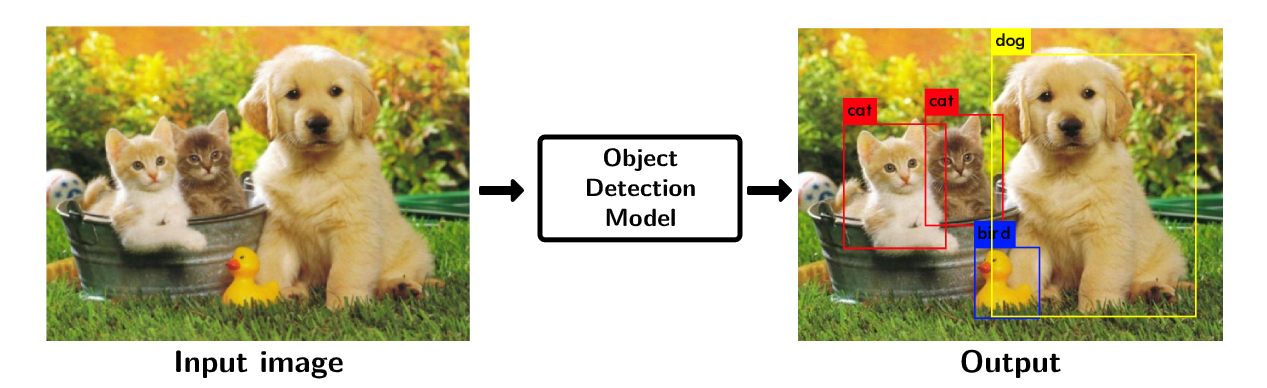
\includegraphics[width=0.9\linewidth]{Sources/Figures/objectdetection.png}
    \caption{A high-level illustration of an object detection pipeline. Adapted
        from \cite{objectdetectionfigure}.}
    \label{fig:od}
\end{figure}

Traditionally, engineers had to hand-craft feature extractors using algorithms
such as SIFT \cite{sift}, SURF \cite{surf}, or HOG \cite{hog}. These methods are
combined with well-established classification algorithms such as Support Vector
Machines (SVM) \cite{svm}. Since this approach needs manual designing, it can be
very demanding.

Deep learning methods introduced an end-to-end learning approach, which means
that the model only takes a given set of annotated images to learn to detect key
features, localize the objects, and classify them. So the hard work is done
mainly by the model itself. This approach outperforms the traditional pipelines
by a significant margin with respect to illumination and viewpoint changes
\cite{outperforming}. We describe deep learning in detail in the Section
\ref{deep_learning_chapter}. But firstly, let us describe how to measure the
performance of object detectors.

\subsection{Evaluation Metrics}
Firstly, let us define evaluation metrics for binary classification. Consider
two classes we want to predict: \bld{positive (P)} and \bld{negative (N)}. Let
\begin{itemize}
    \item \bld{true positives (TP)} be correctly predicted P cases,
    \item \bld{true negatives (TN)} be correctly predicted N cases,
    \item \bld{false negatives (FN)} be all P cases we wrongly predicted as N,
    \item \bld{false positives (FP)} be all N cases we wrongly predicted as P.
\end{itemize}
Suppose we want to focus on the performance of P cases prediction. We define
metrics \bld{precision} and \bld{recall} as follows:
$$
    \text{precision} = \frac{\text{TP}}{\text{TP} + \text{FP}}, \\
    \text{recall} = \frac{\text{TP}}{\text{TP} + \text{FN}}.
$$
Precision is also known as a positive predictive value, i.e., how many of the
positive predictions (TP + FP) actually belong to P class. Recall is known as a
true positive rate and it measures how many TP we have predicted out of all
actual P cases (TP + FN). There is a trade-off relationship between these
metrics. If we increase the precision (e.g., by setting more strict constraints
for assigning TP to a prediction), the recall decreases as there would be more
FN cases, and vice versa.

For an object detection model evaluation, we can suppose that TP represents
correctly detected object. Similarly, FP can be viewed as a wrongly detected
object or duplicate detection. We would like to combine the precision and recall
to a single composite score -- \bld{mean average precision (mAP)}. However,
before we delve into its definition, let us first describe how to determine the
TP and FP from the model's predictions.

\begin{figure}[H]
    \centering
    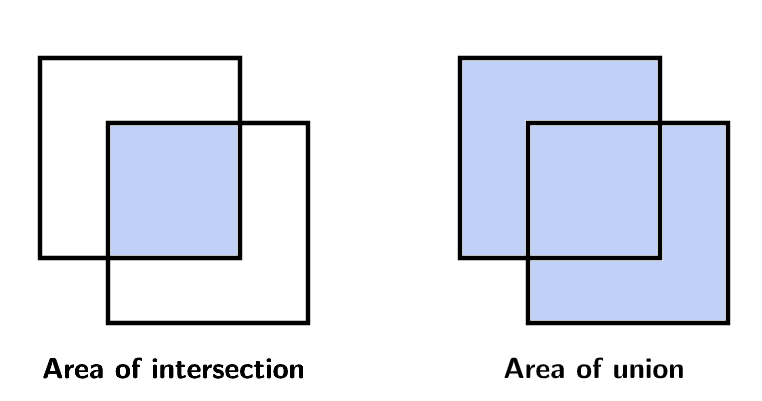
\includegraphics[width=0.6\linewidth]{Sources/Figures/iou.png}
    \caption{Illustration of two bounding boxes and the two types of areas they
        form.}
    \label{fig:iou}
\end{figure}

Models output a list of predictions that are defined by \bld{bounding box}
coordinates (the boundaries of the detected object), \bld{predicted class}, and
\bld{confidence score} of the prediction. To determine if the detection is
correct, we need to define \bld{Intersubsection-over-Union (IoU)}. IoU is
defined as a proportion of the area of intersubsection (overlap between
predicted bounding box and the ground-truth bounding box) and the area of union
(see Figure \ref{fig:iou}):
$$
    \text{IoU} = \frac{\text{area of intersubsection}}{\text{area of union}}.
$$
We simply declare the prediction as a TP if the IoU of the ground-truth bounding
box and the predicted bounding box is greater than a fixed IoU threshold.
Otherwise the prediction is considered as a FP. Now that we know how to determine
the TP and FP cases, we can define mAP.

Mean average precision is an averaged \bld{average precision (AP)} over all
classes. Let us define AP for some class $c$. We denote it as AP$_{c}$. For
illustration, consider a simplified example: we collect all predictions for the
class $c$ from all test images, and we rank them by the confidence score. Let
\bld{positive predictions} be those predictions that have IoU > 0.5. If there
are more positive predictions for a single object, only the prediction with a
higher confidence score is considered to be a TP. See the example Table
\ref{tab:ap}. In the definition of AP, precision is defined as the proportion of
all predictions above the rank which are TP. Whereas recall is defined as the
proportion of TP ranked above a given rank and all positive predictions.
\begin{table}[H]
    \centering
    \begin{threeparttable}
        \begin{tabular}{|c|c|c|c|c|c|}
            \hline
            \bld{rank} & \bld{IoU > 0.5} & \bld{confidence score} & \bld{TP/FP} & \bld{Precision} & \bld{Recall} \\
            \hline
            1          & yes             & 98 \%                  & TP          & 1.00            & 0.2          \\
            2          & yes             & 88 \%                  & FP$^*$      & 0.50            & 0.2          \\
            3          & yes             & 78 \%                  & TP          & 0.67            & 0.4          \\
            4          & yes             & 75 \%                  & TP          & 0.75            & 0.6          \\
            5          & no              & 60 \%                  & FP          & 0.60            & 0.6          \\
            6          & yes             & 59 \%                  & TP          & 0.67            & 0.8          \\
            \hline
        \end{tabular}
        \begin{tablenotes}
            \small
            \item  $^*$ consider this example as a duplicate of the rank 1
            example.
        \end{tablenotes}
        \caption{An example of predictions.}
        \label{tab:ap}
    \end{threeparttable}
\end{table}

Let us explain the calculation behind the third row. The precision is
$2/3 \doteq 0.67$, because there are 2 TP out of 3 predictions above the third
row (including the row). The recall is $2/5 = 0.4$, since there are 2 TP out of
5 positive predictions (IoU > 0.5). As we can see, the precision has a "zigzag"
pattern as we go down the ranking. Whereas the recall is increasing.

The AP$_c$ is defined as an \bld{area under the precision-recall curve} (see
Figure \ref{fig:precisionrecall}). To reduce the impact of the zigzags, we
interpolate the curve at each recall value $r$ by taking the maximum precision
$p_\text{interp}$ measured "to the right":
$$
    p_\text{interp}(r) = \max\limits_{\hat{r}:\hat{r} \geq r} p(\hat{r}),
$$
where $p(\hat{r})$ is the measured precision at the measured recall $\hat{r}$.
We obtain a monotonically decreasing curve that can be numerically integrated as
it is a piecewise constant (see the red dashed curve in Figure
\ref{fig:precisionrecall}). We sample all unique recall values $R$ and compute
AP$_c$ as a sum of rectangular blocks as follows:
$$
    \text{AP}_c = \sum\limits^{\lvert R\rvert - 1}_{n = 0} (r_{n+1} - r_n)
    \cdot p_\text{interp}(r_{n+1}).
$$

\begin{figure}[H]
    \centering
    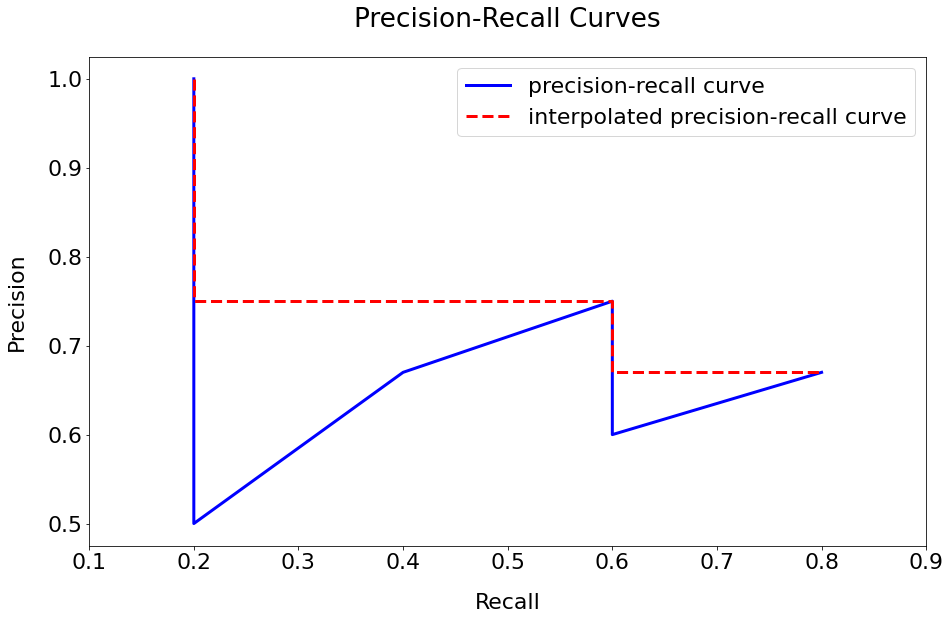
\includegraphics[width=0.8\linewidth]{Sources/Figures/precisionrecall.png}
    \caption{Precision-recall curves.}
    \label{fig:precisionrecall}
\end{figure}

We then get the final mAP by averaging all AP$_c$ for every class (let $C$ be
the set of all classes):
$$
    \text{mAP} = \frac{1}{\lvert C \rvert} \cdot \sum_{ c\in C} \text{AP}_c.
$$
The VOC competitions \cite{voc} used this metric for a fixed IoU = 0.5 threshold.
However, for our evaluation, we use the \bld{updated COCO challenge metric}
\cite{coco} that averages the mAP over 10~different IoU thresholds (from 0.50
to 0.95 with 0.05 step size). We denote it as AP$_{.50:.05:.90}$ = AP.
Similarly, for single IoU thresholds we have AP$_{50}$ (the standard VOC metric)
and AP$_{75}$ (a~strict metric). They also define AP$_\text{small}$,
AP$_\text{medium}$, and AP$_\text{large}$ for varying object's size:
\begin{itemize}
    \item AP$_\text{small}$ is an AP for small objects (bounding box area <
          $32^2$ px),
    \item AP$_\text{medium}$ is an AP for medium objects ($32^2$ px < area <
          $96^2$ px),
    \item AP$_\text{large}$ is an AP for large objects (area > $96^2$ px).
\end{itemize}
Note that they do not make distinction between mAP and AP. Henceforth, whenever
we refer to the AP, we mean the primary COCO metric AP$_{.50:.05:.90}$.

%%%%%%%%%%%%%%%%%%%%%%%%%%%%%%%%%%%%%%%%%%%%%%%%%%%%%%%%%%%%%%%%%%%%%%%%
\section{Deep Learning}\label{deep_learning_chapter}
In this part, we briefly introduce relevant topics of deep learning. For the
sake of readability, we only limit ourselves to high-level and simple
descriptions. The covered concepts are very well described in the book written
by the pioneers of deep learning, Ian Goodfellow, Yoshua Bengio, and Aaron
Courville \cite{Goodfellow-et-al-2016}. In fact, we draw inspiration from the
book for some of our definitions.

The history of artificial neural networks (ANNs) can be dated back to the 1940s
\cite{McCulloch_1943}. However, only since 2006, deep architectures of ANN have
become a trendy area of machine learning research
\cite{DBLP:journals/corr/Schmidhuber14}. That year, Hinton et al. introduced
unsupervised pre-training of deep feedforward neural networks
\cite{hinton2006reducing}. Using this method on a deep belief network
\cite{DBN}, the model achieved 1.2\% error rate on the MNIST classification
dataset \cite{hinton2006fast, mnist}. This exceptional result drew attention
to deep neural networks. The detailed historical development of artificial
neural networks and deep learning is nicely overviewed in a journal article by
another important figure in the field Juergen Schmidhuber
\cite{DBLP:journals/corr/Schmidhuber14}.

\subsection{Deep Feedforward Network}
The fundamental model of deep learning is a \bld{deep feedforward network}, also
known as feedforward neural networks, or multilayer perceptrons. Feedforward
networks approximate arbitrary functions of the form $y = f^*(x;\theta)$, where
$y$ is the \bld{output}, $x$ is the \bld{input}, and $\theta$ are the network's
\bld{weights} (or parameters). For example, in our case, we would like to
output the list of objects with their respective coordinates and classes based
on the input image. The process of finding the best weights $\theta$ for
accurate approximation is called \bld{training} (or the network \bld{learns}).
We describe this process in detail in Section \ref{sec:training}.

The network $f^*$ is composed of intermediate computations that are defined by
some function $f^{(i)}$. We might write the approximated function as a function
composition of $n$ functions:
$$
    f^*(x) = (f^{(n)} \circ f^{(n-1)} \circ ... \circ f^{(2)} \circ f^{(1)})(x).
$$
As we can see, the information flows sequentially in the network; thus, it is
called feedforward. Each of the function $f^{(i)}$ is called \bld{layer}. The
deep learning models are composed of many different layers. We say that the
network is deep; hence, the name \bld{deep learning}. In the next sections, we
describe different types of layers.

\subsection{Convolutional Neural Network}
In the following subsections we describe the layers of \bld{convolutional neural
    networks} that are a special case of a feedforward networks. They thrive at
image processing tasks as a result of a very effective way of feature
extraction.

\subsubsection{Fully-connected Layer}
The most basic layer is \textbf{fully-connected layer} (also known as
\textbf{linear} or \textbf{dense} layer). It performs a transformation from
\textbf{input vector} $\boldsymbol{x}$ of size $m$ into \textbf{output vector}
$\boldsymbol{y}$ of size $n$. The transformation has two parameters, a
\textbf{weight matrix} $\boldsymbol{W}$ of size $m \times n$ and \textbf{bias}
$\boldsymbol{b}$ of size $n$. Firstly, the input vector is weighted by $W$, then
the bias is added, and finally an \textbf{activation function} $\boldsymbol{f}$
is applied to every element (see Section \ref{afunctions} for more details on
activation functions).
$$
    y = f(W\cdot x + b)
$$
See figure \ref{fig:fcl} for a graph representation of a neural network composed
of two fully-connected layers, where each node is a neuron, and each directed
edge is a weight.

\begin{figure}[h]
    \centering
    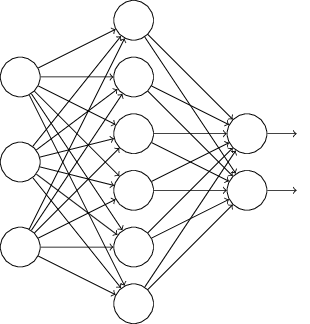
\includegraphics[width=4cm]{Sources/Figures/fully_connected_layer.png}
    \caption{Multilayer Perceptron with two fully-connected layers. Taken from
        \cite{nielsenneural}.}
    \label{fig:fcl}
\end{figure}

\subsubsection{Convolution Layer}
The most important layer of CNNs is the \textbf{convolution layer}. It
introduces a new concept of shared weights, which help us train deeper
architectures and is more suited for image processing tasks. To illustrate the
convolution layer, imagine the input as a square of neurons, i.e., a
two-dimensional \textbf{image} $\boldsymbol{I: (W, H) \rightarrow \real}$
\todo{Zmatecna definice. Sjednotit styl notaci.}, where ${W}$ is the width and
${H}$ is the height of the image.

In contrast with a fully-connected layer, we do not connect every input neuron
to every output neuron. Instead, every output neuron is associated with a
smaller region in the input image. Each association is defined by its
\textbf{bias} $\boldsymbol{b}$ and $\textbf{weights}$ $\boldsymbol{K:(K_w, K_h)
        \rightarrow \real}$, where $K_w$, $K_h$ is the region's width and height. The
output of the layer is a downscaled image $\boldsymbol{Y:(W - K_w + 1,}$
$\boldsymbol{H - K_h + 1)  \rightarrow \real}$, which is often called a
\textbf{feature map}. The value of the $i, j$-th output neuron $Y(i,j)$ is
defined by:
$$
    Y(i, j) = f\left((I * K)(i,j) + b\right)
$$

The $*$ operation is called \textbf{convolution}\todo{Fskutecnosti
    cross-correlation. Doplnit poznamku.} and is defined as follows:

$$
    (I * K)(x, y) = \sum\limits_{k = 1}^{K_w}\sum\limits_{l = 1}^{K_h}
    I(x + k, y + l) \cdot K(k, l)
$$

This process is applied to the whole input image (see figure
\ref{fig:convolution}). The convenience of this method comes with using the same
weights $K$ for each convolution operation. The weights $K$ (and also bias $b$)
are called \textbf{kernel} or \textbf{filter}. The kernel is trained to detect
some non-linear pattern. Therefore, we use multiple kernels to recognize
various features in the image (we end up with multiple feature maps). The
approach also helps CNNs to adapt to image \textbf{translation invariance},
i.e., the detected features do not depend on their positions in the input
image.

For illustration purpose, we have considered a two-dimensional inputs. However,
in practice, we often work with RGB or even RGB-D images represented by
\textbf{tensors} of shape $(W, H, C)$, where $C$ is number of channels (e.g.
three for classic RGB image).

Another important parameter of the layer is \textbf{stride length}. It defines
the number of pixels the filters shifts over the input image. The bigger is
stride length the more downscaled the output image is.

\begin{figure}[h]
    \centering
    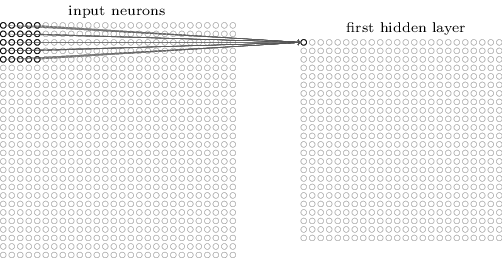
\includegraphics[width=10cm]{Sources/Figures/convolution.png}
    \caption{Illustration of a convolution layer with 5 $\times$ 5 kernel. Taken
        from \cite{nielsenneural}.}
    \label{fig:convolution}
\end{figure}

\subsubsection{Pooling Layer}
Another essential layer for CNNs is the \textbf{pooling layer}. In CNN
architectures, the pooling layers typically come after the convolution layers.
They are used for downscaling the feature maps to reduce the number of network
parameters.

The layer works in a similar manner to the convolution layer. It takes multiple
values from a pooling region and outputs a single pixel. The most common type of
a~ pooling operation is \textbf{max pooling}, which outputs the region's
maximum value. Another operation that can be applied to the region is
\textbf{average pooling}, which outputs the region's mean value.

The pooling region's shape is typically 2 $\times$ 2. In some cases, we want to
pool from the whole input. We call these operations \textbf{global poolings}
(e.g., global max pooling).

\subsubsection{Activation Functions}
\label{afunctions}

Activation functions introduce non-linearity to the layers. Some of the most
important ones are listed below:
\begin{itemize}
    \item \textbf{ReLU} (rectified linear unit) is the most popular activation
          function, which was introduced in \cite{pmlr-v15-glorot11a}. It is defined
          as follows: $\text{ReLU}(x) = \max(0, x)$. It deals better with vanishing
          gradient than sigmoidal functions, which tend to saturates on extreme values.
    \item \textbf{Leaky ReLU} deals with the so-called
          \textbf{dying ReLU problem}. If we use simple ReLU, many neurons cannot
          recover from being stuck at zero value. We can tackle the problem by
          "leaking out" the negative values. The leaked values are then weighted by
          parameter $\alpha$: $\text{Leaky ReLU}(x) = \max(\alpha x, x)$
    \item \textbf{Softmax} funciton is typically used in a last layer of
          classification neural networks. It takes a vector of real numbers and
          normalizes the values into a probability distribution. For input vector
          $x \in \real^K$ and output vector $y \in \real^K$, the function is defined
          as follows:
          $$
              y_i = \text{softmax}(x)_i = \frac{e^{x_i}}{\sum\limits^{K}_{j = 1}
                  e^{x_j}} \text{ for } i = 1,...,K
          $$
\end{itemize}

\subsection{Training}
\label{sec:training}
We find the best weights by minimizing the loss function $\mathcal{L(\theta)}$
that determines the quality of the model with parameters $\theta$. There are
many different loss functions. However, we only describe the most common ones
for classification and regression tasks.

\subsubsection{Loss functions}

\bld{Mean squared error (MSE)} is the most commonly used regression loss
function. It is an average of squared errors. Error is defined as a difference
(or distance) between predicted and actual value. Consider a dataset of $n$
examples $\mathcal{D} = \{(x_i, a_i)\mid i = 1,...,n\}$ where $x_i$ is the input
and $a_i$ is the actual value. Let $y_i = f^*(x_i; \theta)$ be the predicted
output of the model based on the input $x_i$ parametrized by the model's weights
$\theta$. We can then define MSE of dataset $\mathcal{D}$ as follows:
$$
    \text{MSE}_{\mathcal{D}}(\theta) =
    \frac{1}{n}\sum\limits^{n}_{i=1}(y_i - a_i)^2
$$
\bld{Cross-entropy loss (CE)} is widely used for classification tasks. For
simplicity, consider a binary classification where the values are either 1 or 0.
Consider again the dataset $\mathcal{D}$ and predictions $y_i$. The CE is then
defined as:
$$
    \text{CE}_\mathcal{D}(\theta) =
    -\frac{1}{n}\sum\limits_{n=1}^{n} a_i \log(y_i) + (1-a_i)\log(1-y_i)
$$
If we look at the model from a statistical point of view, it learns to capture
the desired probability distribution of some dataset. So the general intuition
behind the CE loss is that it measures the difference between two probability
distributions -- the learned distribution and ground-truth distribution. The
lower the CE is, the more similar the distributions are. Another more precise
mathematical interpretation is that minimizing CE is equivalent to maximizing
the model's maximum likelihood.\footnote{Likelihood function measures the
    goodness of fit of a statistical model to a sample of data for given values
    of the unknown parameters. Definition borrowed from
    \url{https://en.wikipedia.org/wiki/Likelihood_function}.
} The defined CE can be easily extended for multi-class (or categorical)
version.

\subsubsection{Learning algorithm}
The process of finding the best weights is an \bld{optimization problem}. The
goal is to minimize the selected loss function by adjusting the weights
accordingly. The most common optimization algorithm used for training neural
networks is \bld{gradient descent (GD)} and its derivatives. The idea behind GD
is to alter the weights in the \bld{opposite direction of the gradient} of the
loss function (the gradient's direction is the steepest ascent) in an iterative
way.

Since the dataset $\mathcal{D}$ can be very large, we cannnot compute the
gradient straight away. Instead, we sample the prior dataset and update the
weights with the sample's gradient. This method is called \bld{stochastic
    gradient descent (SGD)} and converges faster than GD. The samples are called
\bld{minibatches} and they can be processed at once by vectorization. Let us now
describe the main variations of SGD.

\bld{Stochastic gradient descent.} Let $\mathcal{B} \subseteq \mathcal{D}$ be
the minibatch, $\nabla\mathcal{L_\mathcal{B}(\theta)}$ be the gradient of
$\mathcal{L}_\mathcal{B}(\theta)$, and $\theta_t$ denotes the weights in the
step $t$ (similarly for other variables). The algorithm can be writen as:
$$
    \begin{array}{rl}
        \Delta\theta_{t} & = - \epsilon_{t} \cdot \nabla{\mathcal{L}_\mathcal{B}(\theta_{t})} \\
        \theta_{t+1}     & = \theta_{t} + \Delta\theta_{t}
    \end{array}
    \quad \text{ for steps } t = 1,2,...
$$
The $0 < \epsilon \leq 1$ is called $\bld{learning rate}$ that controls the
speed of model's learning. In plain SGD, the $\epsilon_t$ is fixed for every
$t$. However, naturally, we want the model to learn faster in the beginning and
slower as it converges and stabilize. The most straightforward way to do so, is
to make use of a learning rate scheduler that alters the $\epsilon$ w.r.t. time.
A more robust way is to change the $\epsilon$ in an \bld{adaptive} way. We want
to have larger rates for smaller updates and smalelr rates for larger updates.
The most common examples of this approach is \bld{AdaGrad} \cite{adagrad},
\bld{AdaDelta} \cite{adadelta}, \bld{RMSProp}.\footnote{It was not published.
    However, it was proposed in a course by Geoff Hinton \url{
        http://www.cs.toronto.edu/~tijmen/csc321/slides/lecture_slides_lec6.pdf}
}

Another way to speed up the SGD is to stabilize the direction of the descent as
it can oscillate. We add a \bld{momentum} to the new weights $\theta_{t+1}$ in
the form of the previous update $\Delta\theta_{t-1}$ additionally to the
$\Delta\theta_{t}$. This extension also helps to escape local minima. Finally,
we would like to mention that the currently suggested optmization algorithm is
\bld{Adam} \cite{adam} that effectively combines the both approaches (adaptive
learning rate and momentum).

\subsubsection{Backpropagation}
Consider $\theta$ to be composed of $m$ weights $\theta = (w_1, w_2, ..., w_m)$.
Let us simplify the notation for $\loss_\mathcal{D}(\theta) = \loss$. Then the
gradient is computed as:
$$
    \grad = \left(\pd{1}, \pd{2}, ..., \pd{m}\right)
$$
where $\partial \loss / \partial w_i$ is a partial derivative of $\loss$ with
respect to $w_i$. Recall that the networks can be represented as a function
composition. Computing the gradients naively by the definition for every $w_i$
is very inefficient as it results in many recomputations due to the chain rule
of derivatives. The \bld{backpropagation} algorithm \cite{backprop} computes the
gradient effectively by computing the gradient backward from the last layer in
the network iteratively layer by layer. This way the recurring subexpressions in
the chain rule are already precomputed.\footnote{This is in fact an example of a
    dynamic programming.}

% can visualize such a composition as a computational graph (see Figure). The
% computation of gradient as it is defined is very inefficient because of
% recurring subexpressions. Let us demonstrate the problem on a simplified graph
% in Figure . Let $a \in \real$ be an input of the graph, a function we apply at
% every step $f: \real \to \real$ of the sequence $b=f(a)$, $c=f(b)$, and
% $d=f(c)$.
% \[\arraycolsep=1.4pt\def\arraystretch{2.2}
%     \begin{array}{rl}
%         \grad  & = \left(\pd{1}, \pd{2}, ..., \pd{m}\right)                   \\
%         \pd{i} & = \mathlarger{\sum\limits_{(x_j, a_j) \in \mathcal{D}}} \pdj 
%         \quad \text{where } \loss_j \text{ is loss function for }
%     \end{array}
% \]

% \centering
% \begin{tikzpicture}[auto]
%     \tikzset{vertex/.style = {shape=circle,draw,minimum size=1.5em}}
%     \tikzset{edge/.style = {->,> = latex'}}
%     % vertices
%     \node[vertex] (1) at  (0,0) {$w_1$};
%     \node[vertex] (2) at  (2,0) {$w_2$};
%     \node[vertex] (3) at  (4,0) {$w_3$};
%     \node (4) at  (6,0) {$\loss$};
%     %edges
%     \draw[edge] (1) to (2);
%     \draw[edge] (2) to (3);
%     \draw[edge] (3) to (4);
% \end{tikzpicture}
% \[\arraycolsep=1.4pt\def\arraystretch{2.2}
%     \begin{array}{rl}
%         \pd{3} & = ...                   \\
%         \pd{2} & = \pd{3} \prt{w_3}{w_2} \\
%         \pd{1} & = \pd{2} \prt{w_2}{w_1}
%     \end{array}
% \]

% consists of partial derivatives $\pderivative$ for every $w_i$. Each
% $\pderivative$ is computed as
% $\pderivative = \sum\limits_{j=1}^{\lvert\mathcal{B}\rvert}$.

\subsection{Overfitting and underfitting}

When we train a machine learning model, we typically have a
\textbf{training set} and a \textbf{test set}. We then fit the model's
parameters on a training set to \textbf{minimize} an error measure
(a \textbf{training loss} or \textbf{error}). However, at the same time, we want
to minimize a \textbf{test error} as well. We say that a model should
\textbf{generalize}. This means that it should perform well on unseen data.

These efforts can lead to two major problems in machine learning. If we train
for too long, the model will learn the training set patterns that do not
generalize to the test set. We say that the model \textbf{overfits}. The
opposite of overfitting is \textbf{underfitting}. It occurs when the model is
not able to gain sufficiently low training loss. Underfitting can happen because
of using a weak model or not training long enough. If we plot the losses, we
want to make sure that the training loss is reasonably low, and the gap between
training and test error is small (see figure \ref{fig:loss_plot}).

\begin{figure}[h]
    \centering
    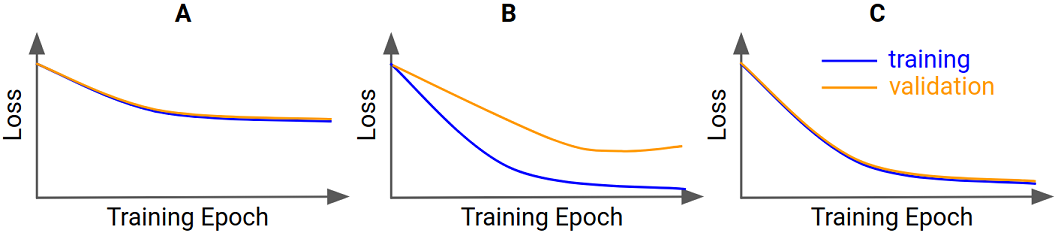
\includegraphics[width=\linewidth]{Sources/Figures/fitting.png}
    \caption{A simplified cases of loss curves showing:
        (A) Underfitting, (B) Overfitting and (C) Optimal fit where validation
        set is unobserved data. Taken from
        \cite{bileschi2020deep}.}
    \label{fig:loss_plot}
\end{figure}

In coming subsections we describe the most common techniques to prevent
overfitting in neural networks.

\subsubsection{$L_2$ Regularization}
Following the Occam's razor principle,\footnote{The simplest explanation is most
    likely the right one.} the extreme weights are likely to cause overfitting. We
can reduce the overfitting by penalizing these weights with $\boldsymbol{L_2}$
\textbf{regularization}. The penalization is performed by adding a $L_2$ term to
the loss function. The term is defined as a sum of squares of weight values.

\subsubsection{Dropout}
Another common technique is called \textbf{dropout}. This method prevents
individual nodes in the network to rely on the output of other nodes by randomly
"dropping out" or "deactivating" some of the neurons. The method's parameter is
a number between 0 and 1 that defines the fraction of the input units to drop.

\subsubsection{Batch Normalization}
Deep neural networks often suffer from unstability. Small changes in layers
close to the input amplify as they propagate through the network. The deeper
layers have to adapt significantly and thus learn slowly.
\textbf{Batch normalization} introduces a way to stabilize and accelerate the
training speed by normalizing the outputs of previous layer by subtracting the
batch mean and dividing by the batch standard deviation.

\subsubsection{Data Augmentation}
The most obvious way to train a robust model is to have an extensive dataset.
However, in some cases, it is very challenging to acquire sufficient ammount of
data. We can overcome this issue by
\textbf{augmenting} the training set by generating new artificial data. Of
course, it is impossible to adopt this approach to every type of datasets, but
it is straightforward for object detection tasks. The simplest way to augment
the image dataset is by adding \textbf{random transformations} (cropping,
resizing, rotation, ...) of the original images. The more sophisticated method
would be generating new \textbf{synthetic} images. With recent advances in
generative adversarial networks (GANs), it is possible to synthesize
high-quality images. An impressive adoption of this approach is proposed in
\cite{wei2019generative}.